\chapter{Opis technologii i aplikacji}

Częśc wymagań wobec tej pracy dotyczyła nie tylko algorytmów i procesu rozpoznawania
tęczówki, ale także sposobu w jaki aplikacja została stworzona i w jaki sposób jest
ona użytkowana. Aplikacja miała by przyjazna dla użytkowników i pozwala\'c na działanie
w trybie krokowym. Miała pozwala\'c również na proste rozszerzanie jej o kolejne
metody. Wymagania te w duży sposób wpłynęły na wybór technologii użytych w tej pracy,
które opisane zostaną w dalszej części tego rozdziału.

\section{Użyte technologie}

Ponieważ praca jest ściśle związana z przetwarzaniem obrazu, w tym wypadku obrazu oka
w celu analizy tęczówki, zdecydowano się na użycie biblioteki OpenCV. Upraszcza ona pracę
z obrazem oraz operacje na nim w znacznym stopniu, a także dostarcza wiele gotowych
funkcji, które przyspieszają tempo tworzenia eplikacji.\newline

Dużą wagę w pracy należało poświęci\'c części klienckiej, w celu stworzenia przejrzystego i
przyjaznego interfejsu użytkownika. Wiele aplikacji zaniedbuje ten aspekt, w wyniku czego
użytkownicy często gubią się w trakcie korzystania z aplikacji. Problem ten najczęściej próbuje
się maskowa\'c przygotowaniem rozległej dokumentacji aplikacji i jej widoków, co nie poprawia
w żaden sposób jakości korzystania z niej. Problemy te prowadzą do zniechęcenia i gorszej jakości
doświadczenia użytkownika, co końcowo prowadzi do zaprzestania korzystania z aplikacji. Aby
unikną\'c tych problemów postanowiono wykorzysta\'c technologie pozwalające na tworzenie
zachęcających i interaktywnych interfejsów. Najlepiej w tym obszarze sprawdzają się technologie
internetowe takie jak HTML (HyperText Markup Language), CSS (Cascading Style Sheets) oraz JS
(JavaScript).

Technologie te nie dają bezpośredniej możliwości użycia w nich bilbioteki OpenCV, nastomiast
możliwe jest stworzenie dodatkowej warstwy, która wykonywałaby przetwarzanie obrazu z
użyciem OpenCV, a następnie komunikowałaby się z interfejsem i przekazywała do niego
wymagane dane. W związku z tym w pracy postanowiono uży\'c języka Python, który dostarcza wielu
rozwiązań umożliwiających taką komunikację.\newline

Zaprojektowanie aplikacji w ten sposób pozwala na rozdzielenie jej na warstwę prezentacyjną
oraz warstwę logiki aplikacyjnej, co jest zgodne z dobrymi praktykami tworzenia oprogramowania.
Pozwala to również na uniezależnienie tych warstw od siebie, dzięki czemu możliwe
byłoby stworzenie wielu interfejsów korzystających z tego samego procesu przetwarzania obrazu.

\subsection{Warstwa logiki aplikacji}

Tak jak wcześniej wspomniano jako główny język programowania odpowiedzialny za warstwę logiki
aplikacji, przetwarzanie obrazu oraz komunikację z interfejsem użytkownika wybrany został język
Python w parze z biblioteką OpenCV.

Tworzenie aplikacji internetowych z wykorzystaniem języka Python bez żadnej dodatkowej
biblioteki byłoby zadaniem żmudnym oraz nie dostarczajacym żadnej dodatkowej wartości. W związaku
z tym zdecydowano się na użycie biblioteki \textbf{Flask}, która dostarcza gotowych rozwiązań
w świecie aplikacji internetowych, upraszcza projetkowanie systemu oraz dostarcza prosty w obsłudze
sposób na komunikację z interfejsem użytkownika. Dodatkowo razem z biblioteką dostarczany jest
deweloperski serwer WWW, dzięki czemu nie trzeba instalowa\'c i konfigurowa\'c żadnych innych zależności.
\newline

Najpopularniejszym sposobem komunikacji między serwerem a interfejsem użytkownika jest zaprojektowanie
interfejsu programistycznego wykorzystującego protokół HTTP w architekturze REST (Representational State Transfer).
Jego zadaniem jest zapewnienie aplikacji klienckiej zestawu usług wykonujących ściśle określone
operacje zależne od użytej metody protokołu HTTP. REST zakłada, że każda z takich usług jest bezstanowa, a wynik jej działania jest w całości
oparty o dane przychodzące wraz z zapytaniem. Każda z usług ma swój unikalny identyfikator w postaci
adresu URL (Uniform Resource Locator) pod który aplikacja kliencka może wysyła\'c zapytania.

Korzystanie z architektury REST wymusza dobre praktyki projektowania interfejsów programistycznych
i jest lubianym wzorcem wśród programistów aplikacji internetowych ze względu na przejrzystoś\'c
tworzonego kodu oraz poniekąd samodokumentujący się kod.
W konteście aplikacji tworzonej w ramach niniejszej pracy, zastosowanie architektury REST pozwala
na rozbicie całego procesu rozpoznawania tęczówki na mniejsze kroki odpowiadające poszczególnym
etapom procesu lub nawet poszczególnym algorytmom. Takie rozbicie można uzyska\'c przez zdefiniowanie
osobnej usługi dla każdego z zaimplementowanych algorytmów. Takie rozwiązanie zapewnia prostą skalowalnoś\'c,
ponieważ dodanie kolejnego algorytmu wymaga jedynie dodania nowej usługi oraz zmiany adresu pod który
wysyłane jest zapytanie.

Biorąc pod uwagę te zalety w pracy zdecydowano
się na użycie \textbf{Flask-RESTful}, które jest rozszerzeniem dla biblioteki Flask. Dostarcza
ono szereg metod i uproszczeń w tworzeniu interfejsów w architekturze REST.\newline

Oprócz wyżej wymienionych bibliotek należy zainstalowa\'c również wszelkie ich zależności, takie jak
przykładowo biblioteka \textbf{Numpy} w przypadku OpenCV. Wraz z rozwojem aplikacji iloś\'c użytych
bibliotek i zależności będzie tylko rosną\'c, co w dłuższym czasie spowoduje problemy z utrzymaniem
informacji o tym jakie biblioteki i które ich wersje są wymagane do uruchomienia aplikacji. Często
informacje te przechowywane są w postaci pliku tekstowego w katalogu projektu, jednak rozwiązanie to
jest mało odporne na błąd ludzki, ponieważ nie trudno zapomnie\'c o aktualizacji takiego pliku.

Dodatkowo pracując jednocześnie przy kilku projektach w języku Python może okaza\'c się, że kilka z
nich wymaga dokładnie tej samej biblioteki, ale w różnych wersjach. Problem ten można rozwiąza\'c
używając wirtualnych środowisk. Są to środowiska Pythona, które są odizolowane i niezależne od głównej
instalacji Pythona. W rzeczywistości są to osobne foldery, w których instalowana jest odpowiednia wersja
Pythona oraz wymagane biblioteki w odpowiednich wersjach.

W celu rozwiązania tych problemów w pracy zdecydowano się na użycie narzędzia \textbf{Pipenv}.
Umożliwia ono automatyczną generację writualnego środowiska wewnątrz projektu oraz automatyczne
śledzenie zależności projektu i ich wersji. Informacje te przechowywane są w dwóch plikach
\textit{Pipfile} oraz \textit{Pipfile.lock}, które są generowane, czytane oraz utrzymywane automatycznie.
Poniżej przestawiono podstawowe komendy narzędzia Pipenv:

\begin{description}
  \item[pipenv install] - uruchomienie w katalogu projektu inicjalizuje środowisko wirtualne oraz pliki
  \textit{Pipfile} i \textit{Pipfile.lock}

  \item[pipenv install <packageName>] - instaluje paczkę wewnątrz środowiska wirtualnego

  \item[pipenv shell] - uruchamia powłokę w której dostępny jest python oraz biblioteki zainstalowane
  w środowisku wirutalnym
\end{description}

\subsection{Warstwa prezentacyjna}

Tak jak wcześniej wspomniano, aplikacja kliencka napisana została z wykorzystaniem technologii
internetowych takich jak HTML, CSS oraz JS. Aplikacje korzystające z tych technologii historycznie
zwykle używane były wewnątrz przeglądarek. W ostatnich czasach technologie internetowe zyskują
coraz większą popularnoś\'c, co przełożyło się również na rozwój dostępnych bibliotek oraz zwiększenie
zasięgu problemów rozwiązywanych tymi technologiami.

Obecnie aplikacje internetowe mogą przyjmowa\'c nie tylko posta\'c stron internetowych, ale także
zwyczajnych, wieloplatformowych aplikacji desktopowych dzięki takim narzędziom jak użyty w niniejszej
pracy \textbf{Electron}. Jest to biblioteka, która używa NodeJS oraz Chromium do stworzenia jednolitego
środowiska uruchomieniowego. Dzięki takiemu połączeniu możliwe jest wygenerowanie okna aplikacji, które
w rzeczywistości jest procesem Chromium przedstawiającym konkretną stronę internetową. Dodatkowo wykorzystanie
NodeJS pozwala na dostęp oraz modyfikację systemu plików użytkownika aplikacji, dzięki czemu możliwe przetwarzanie,
usuwanie i modyfikowanie plików bez potrzeby przeysłania ich na jakikolwiek serwer. Jest to nieosiągalne
przy użyciu przeglądarkowej implementacji języka JavaScript.\newline

Tworzenie aplikacji korzystając z podstawowych możliwości HTML, CSS oraz JS zapewne zajęłoby
bardzo dużo czasu, dlatego w świecie technologii internetowych powstaje wiele bibliotek
ułatwiających tworzenie skomplikowanych i interaktywnych aplikacji. Jedną z nich jest
\textbf{React}, który został użyty w tej pracy. Jest to biblioteka JavaScript umożliwiająca
tworzenie interfejsów użytkownika. Każdy interfejs można rozłoży\'c na poszczególne bloki
odpowiadające za pewną funkcjonalnoś\'c np. wyświetlenie obrazu, zebranie danych od użytkownika,
czy przełączenie między dwoma widokami. Bloki te nazywa się komponentami i mogą by\'c one wykorzystywane
wielokrotnie w różnych miejscach aplikacji. Tworzenie reużywalnych komponentów jest podstawą
biblioteki React, co sprawia, że jest ona idealnym kandydatem do zbudowania interfejsu aplikacji
niniejszej pracy.\newline

Komponenty powinny by\'c w miarę możliwości od siebie niezależne, a ich implementacja powinna
dokonywa\'c jedynie operacji wymaganych właśnie przez ten komponent. Każdy z komponentów cechuje
pojęcie stanu - informacji opisujących stan komponentu w danym momencie. W momencie, gdy komponent
nie jest wyświetlany, jest on niszczony, a wraz z nim jego stan, co pozwala na zwolnienie
zajętej pamięci. Istnieją natomiast informacje, które są ważne dla działania całej aplikacji, z których
korzysta wiele różnych komponentów w celu wyświetlenia danych, w związku z czym muszą by\'c przechowywane
przez cały cykl życia aplikacji. Dokładnie taki przypadek można zaobserwowa\'c w niniejszej pracy, np.
informacje o segmentacji obrazu tęczówki potrzebne będą nie tylko w celu wyświetlenia tych danych,
ale także w celu wykorzystania ich w kolejnych etapach procesu przetwarzania. Do przechowywania danych
poza komponentami użyta została biblioteka \textbf{Redux}.

Jednym z wymogów postawionych przed aplikacją jest działanie w dwóch trybach: krokowym oraz wsadowym.
Każdy z tych trybów składa się z kilku kroków, np. tryb krokowy składa się z następujących kroków:

\begin{itemize}
  \item wybór przetwarzanego obrazu,
  \item przetwarzanie wstępne,
  \item segmentacja,
  \item normalizacja,
  \item kodowanie,
  \item wybór obrazów do procesu dopasowania,
  \item dopasowanie,
  \item prezentacja wyników.
\end{itemize}

Dla każdego z tych kroków konieczne będzie stworzenie innego widoku, ponieważ każdy z nich będzie wyglądał
nieco inaczej. W aplikacji złożonej z tak wielu widoków prosto o problemy związane z przejściami między nimi,
które mogą skutkowa\'c nieprzewidywalnymi błędami, np. załadowanie widoku normalizacji przed widokiem segmentacji
może skutkowa\'c błędem krytycznym aplikacji. W celu uniknięcia takich błędów interfejs użytkownika można
opisa\'c w postaci automatu skończonego, w którym stanami są poszczególne widoki, a zmiana widoku definiowana
jest przez odpowiednie przejścia. Zapewnia to przewidywalnoś\'c działania systemu i uodparnia go na
błedy podobne do tych wspomnianych wcześniej. W celu opisu interfejsu aplikacji za pomocą automatu skończonego
wykorzystana została biblioteka \textbf{xState}.\newline

Częś\'c komponentów, która tworzy aplikację jest bardzo uniwersalna i powszechna w wielu innych zastosowaniach.
Są to komponentu typu \textit{przycisk, link, lista elementów, tabela, ikona}. W związku z ich powszechnością
powstało wiele bibliotek gotowych komponentów, dzięki czemu tworząc aplikację można skupi\'c się na logice
biznesowej stojącej za aplikacją, zamiast na nowo implementowa\'c przykładowo działanie przycisku. Większoś\'c
z tych bibliotek dodatkowo zapewnia podstawowe style, dzięki czemu aplikacje tworzone z ich wykorzystaniem
wymagają mniejszego nakładu pracy, by aplikacja wyglądała zachęcająco. Aby zmniejszy\'c potrzebny nakład
pracy do wytworzenia interfejsu użytkownika, w pracy użyta została biblioteka komponentów \textbf{Ant Design}.
\newline

Podobnie jak w przypadku Pythona, iloś\'c bibliotek i narzędzi używanych w ramach aplikacji jest bardzo duża,
a manualne utrzymywanie informacji o nich oraz ich wersjach byłoby niemożliwe. W związku z tym wykorzystany
został menadżer pakietów \textbf{Yarn} umożliwiający prostą instalację bibliotek i narzędzi, który automatycznie
zapisuje zainstalowane paczki oraz ich wersje jako zależności projektu w plikach \textit{package.json} oraz
\textit{yarn.lock}. Dzięki korzystaniu z Yarna wszystkie zależności i biblioteki można zainstalowa\'c wywołując
w folderze zawierającym plik \textit{package.json} komendę \texttt{yarn install}.

W ramach pracy wykorzystane zostały również inne narzędzia, do których wyboru przyczyniła się wyłącznie
osobista preferencja:

\begin{description}
  \item[Babel] - kompiler JavaScript, pozwalający na korzystanie z najnowszych oraz testowych funkcjonalności
  JavaScript przez transformację kodu \'zródłowego w nowszej wersji do kodu wynikowego w starszej wersji.
  \item[Styled Components] - biblioteka pozwalająca na definiowanie styli CSS dla poszczególnych komponentów
  w plikach \'zródłowych o rozszerzeniu \textit{*.js}.
  \item[Webpack] - narzędzie uruchamiające kompilatory kodu \'zródłowego przekształcające go do postaci rozumianej
  przez przeglądarki oraz łączące wiele plików w pojedyńczy plik wynikowy.
  \item[Axios] - biblioteka ułatwiająca wysyłanie zapytań do serwera.
\end{description}

\subsection{Inne technologie}

Podczas pracy nad projektem używany był system kontroli wersji Git. W trakcie programowania
często zachodzi potrzeba zmiany istniejącego i działającego kodu w celu dodania nowych funkcjonalności.
Niezapisanie poprzedniej wersji kodu może skutkowa\'c niemożliwością powrotu do wersji przed
wprowadzeniem zmian, tym samym generując dodatkową pracę wymaganą do naprawienia powstałych
problemów. System kontroli wersji Git pozwala na zapisanie aktualnego stanu pracy w dowolnym momencie.
Dzięki temu wprowadzanie zmian w działającym kodzie jest znacznie mniej ryzykowne, ze względu na
możliwoś\'c powrotu do dowolnej poprzedniej wersji. Korzystając z tego systemu kontroli wersji uzyskujemy
również dostęp do historii poszczególnych plików, a także możliwoś\'c dodawania komentarzy podczas zapisywania nowych wersji,
dzięki czemu łatwiej zrozumie\'c co dane zmiany robią i dlaczego zostały wprowadzone.

Dodatkowym atutem jest możliwoś\'c przechowywania całości projektu w zewnętrznym serwisie. Dzięki
temu w razie awarii sprzętu, na którym tworzony jest projekt, w najgorszym wypadku stracona
zostanie jedynie częś\'c pracy, a nie jej całoś\'c.

\section{Struktura kodu}

Struktura projektu podzielona została na trzy główne foldery:

\begin{itemize}
  \item \textbf{/app} - zawiera kod \'zródłowy oraz konfiguracje narzędzi użytych przez aplikację
  kliencką,
  \item \textbf{/sever} - zawiera kod \'zródłowy oraz konfigurację narzędzi użytych przez aplikację
  serwerową dokonującej przetwarzania tęczówki,
  \item \textbf{/thesis} - zawiera kod \'zródłowy pracy dyplomowej w formacie \textit{*.tex}
\end{itemize}

Używając takiego podziału, łatwo odnale\'z\'c miejsce odpowiadające za szukaną funkcjonalnoś\'c.
W głównym folderze projektu znajduje się również plik \textit{README.md}, w którym opisane zostały
instrukcje dotyczące uruchomienia projektu.

\subsection{Struktura projektu aplikacji klienckiej}

\begin{itemize}
  \item \textbf{/dist} - zawiera kod wynikowy wygenerowany przez Webpack,
  \item \textbf{/src/js} - zawiera kod \'zródłowy napisany w JavaScript,
  \begin{itemize}
    \item \textbf{actions} - folder dla akcji używanych przez bibliotekę Redux,
    \item \textbf{api} - folder zawierający funkcje pomocnicze wysyłające zapytania do serwera o odpowiednie algorytmy
    przetwarzania tęczówki,
    \item \textbf{components} - folder zawierający komponenty uniwersalne dla całej aplikacji,
    \item \textbf{constants} - folder zawierający pliki eksportujący stałe używane przez resztę kodu,
    \item \textbf{helpers} - folder zawierający funkcje pomocnicze,
    \item \textbf{reducers} - folder w którym definiowane są konsekwencje akcji (Redux)
    \item \textbf{stateMachine} - folder w którym znajduje się opis interfejsu użytkownika za pomocą
    maszyny stanów (xState)
    \item \textbf{store} - folder definiujący scentralizowany stan aplikacji (Redux)
    \item \textbf{views} - folder zawierający implementacje poszczególnych widoków dla obu trybów działania aplikacji
  \end{itemize}
  \item \textbf{/webpack} - zawiera pliki konfiguracyjne Webpacka opisujące sposób przetwarzania kodu \'zródłowego.
\end{itemize}

\subsection{Struktura projektu aplikacji serwerowej}

\begin{itemize}
  \item \textbf{/.venv} - folder zawierający wirtualne środowisko projektu wraz z potrzebnymi
  bibliotekami,
  \item \textbf{/const} - folder zawierający stałe używane przez resztę kodu,
  \item \textbf{/processing} - folder zawierający implementacje algorytmów dla poszczególnych etapów
  procesu,
  \item \textbf{/resources} - folder zawierający kod definiujący strukturę stworzonego API,
  kod eksponujący na zewnątrz algorytmy zaimplementowane w folderze \textit{processing},
  \item \textbf{/temp} - folder tymczasowy zawierający wyniki etapów procesu w postaci zdję\'c,
  \item \textbf{/utils} - folder zawierający funkcje pomocnicze.
\end{itemize}

\section{Działanie aplikacji}

W tej części rozdziału przedstawiony zostanie opis interfejsu użytkownika za pomocą
maszyny stanów, a także opisane zostaną poszczególne widoki aplikacji oraz jej możliwości.

\subsection{Opis interfejsu aplikacji}

\noindent Wszystkie zrzuty ekranu aplikacji, do których odwołuje się poniższy opis można znale\'z\'c w dodatku
\ref{appendix:appScreenShots} na stronach \pageref{fig:homeScreen} - \pageref{fig:batchSingleEntryResult}. \newline

\vspace{-20pt}
\paragraph{Tryb krokowy\newline}

Po uruchomieniu aplikacji oczom użytkownika ukazuje się ekran startowy \ref{fig:homeScreen} witający użytkownika
i proszący go o wybranie jednego z dwóch trybów działania aplikacji.\newline

Wybranie trybu krokowego przenosi użytkownika do kreatora, który przeprowadzi go przez proces
rozpoznawania tęczówki. Wszystkie kroki kreatora widoczne są w górnej części widoku. Aktywny krok
jest zawsze oznaczony kolorem niebieskim. Pierwszym krokiem kreatora jest wybranie obrazu, który chcemy
podda\'c przetwarzaniu (rysunek \ref{fig:processingImageSelectionScreen}). W celu wyboru użytkownik może klikną\'c w wyświetlone pole lub
przeciągną\'c na nie wybrany obraz. Po lewo od kreatora znajduje się rozwijane menu, które
pozwala użytkonikowi na przełączenie się w inny tryb lub przejście do ekranu domowego w każdym
momencie działania aplikacji. Przejście pomiędzy trybami jest równoznaczne z wykasowaniem
dotychczasowo wybranych informacji w poprzednio aktywnym trybie.

Kliknięcie przycisku ``Next'' spowoduje przejście do kolejnego kroku kreatora Jeżeli użytkownik
nie wybrał obrazu, kreator nie przejdzie do następnego kroku i poinformuje użytkownika o konieczności
wyboru obrazu.\newline

Następnym krokiem kreatora jest przetwarzanie wstępne (rysunek \ref{fig:preprocessingScreen}). Widok ten
przedstawia użytkownikowi obecny stan wybranego obrazu po lewej stronie oraz formularz pozwalający
na kontrolowanie metody przetwarzania i jej paramterów po prawej stronie. Pod obrazem dostępny jest
przycisk ``Save", którego kliknięcie poprosi użytkownika o wybranie miejsca, w którym wyświetlony obraz
ma zosta\'c zapisany. Kliknięcie przycisku ``Process'' znajdującego się pod formularzem skutkuje
zaaplikowaniem wybranego algorytmu z wybranymi parametrami. Jeżeli przycisk ``Process'' został wciśnięty
chociaż jeden raz, to pojawi się przycisk ``Revert last'', którego kliknięcie powoduje cofnięcie się
do poprzedniego stanu obrazu. Zmiana wybranego algorytmu skutkuje również zmianą dostępnych
do modyfikacji paramterów (rysunek \ref{fig:preprocessingOtherMethod}).

Na samym dole widoku dostępne są dwa przyciski. Przycisk ``Next'', podobnie
jak poprzednio, powoduje przejście do następnego kroku kreatora, a przycisk ``Previous'' do poprzedniego
kroku kreatora. Przejście do poprzedniego kroku kasuje wszelkie zapisane informacje związane z aktualnym
krokiem. W tym kroku kreatora możliwe jest przejście do kolejnego kroku nie uruchamiając żadnego z
algorytmów przetwarzania wstępnego.\newline

Kolejne kroki kreatora funkcjonują w bardzo podobny sposób. Różnicą może by\'c iloś\'c wyświetlanych
obrazów. Jeżeli wymagane jest wyświetlenie informacji o kilku obrazach, to prezentowane są one w formie
zakładek. Sytuację taką można zaobserwowa\'c w widoku procesu normalizacji (rysunek \ref{fig:normScreen}),
gdzie możliwy jest podgląd przed i po normalizacji oryginalnego obrazu, maski oraz maski nałożonej na
zdjęcie.\newline

Następnie przechodzimy do kodowania, którego widok ma taką samą strukturę jak widoki przetwarzania
wstępnego czy normalizacji, ale pozwala na podgląd innych obrazów oraz na wybór innych metod.\newline

Kolejnym krokiem po kodowaniu jest wybór obrazów, do których chcemy spróbowa\'c dopasowa\'c obraz
wybrany w kroku pierwszym (rysunek \ref{fig:matchingImagesScreen}). W celu wyboru obrazu należy
uży\'c przycisku znajdującego się w górnej częsci ekranu. Możliwe jest wybranie wielu obrazów na raz.\newline

Po zatwierdzeniu obrazów użytkownik zostaje przeniesiony do widoku dopasowania, gdzie ponownie
może wybra\'c metodę oraz jej parametry. Kliknięcie przycisku ``Next'' w tym widoku
uruchamia proces, na który składa się przetworzenie wszystkich wybranych obrazów w dokładnie
ten sam sposób, co obraz wybrany w kroku pierwszym oraz przeprowadzenie operacji dopasowania.
Ponieważ przetwarzanie kilku obrazów może potrwa\'c pewien czas, użytkownik przenoszony jest do
nowego ekranu (rysunek \ref{fig:matchingProcessing}), gdzie wyświetlana jest mu informacja o obecnym
stanie aplikacji wraz z animowaną ikoną, która zapewnia, że aplikacja nie zacięła się.

W wypadku, gdy przetwarzanie zostanie przerwane z powodu błędu, użytkownik przeniesiony zostanie do ekranu
dopasowania. Jeżeli natomiast przetwarzanie zakończy się sukcesem, użytkownik przeniesiony zostanie
do widoku prezentującego wyniki \ref{fig:stepResultsScreen}. Pierwszym z elementów tego widoku
jest przycisk umożliwiający zapisanie konfiguracji użytej do przetworzenia obrazów w postaci pliku
o rozszerzeniu JSON (JavaScript Object Notation), który może zosta\'c użyty pó\'zniej w trybie
wsadowym. Plik ten ma następującą strukturę:

\begin{verbatim}
  {
    "PREPROCESSING":[
      {
        "method":"GAUSS",
        "methodParams":{
          "kernelWidth":3,
          "kernelHeight":3,
          "sigmaX":0,
          "sigmaY":0,
        }
      }
    ],
    "SEGMENTATION":{
       "segmentationMethod":"Daugman",
       "noiseMethod":"none"
    },
    "NORMALIZATION":{
       "method":"DAUGMAN",
       "methodParams":{
          "width":260,
          "height":32
       }
    },
    "ENCODING":{
       "method":"LOG_GABOR",
       "methodParams":{
          "minWaveLength":18,
          "sigmaOnf":0.5
       }
    },
    "MATCHING":{
       "method":"HAMMING",
       "methodParams":{
          "acceptedHammingDist":0.35,
          "shiftsNumber":8
       }
    }
 }
\end{verbatim}

Zapisanie konfiguracji procesu do pliku pozwala użytkownikowi na eksperymentację z wartościami poszczególnych
paramterów w trybie krokowym, a nastepnie przejście do trybu wsadowego, gdzie może przeprowadzi\'c ten proces
dla większego zbioru obrazów.\newline

Poniżej przycisku zapisującego konfigurację wyświetlane są informacje o wynikach dopasowania
dla poszczególnych obrazów. Pokazują one podstawowe informacje, tj.: ścieżki do plików,
miniaturki obrazów oraz wynik dopasowania. Jeżeli użytkownik chce pozna\'c więcej szczegółów, może
uży\'c przycisku ``See more''. Kliknięcie go powoduje otwarcie nowego okna dialogowego, w którym
przedstawione zostaje dokładniejsze zestawienie danych (rysunek \ref{fig:stepResultPreview}).
W lewym górnym rogu prezentowane są informacje o etapie dopasowania. Wyświetlana jest informacja
o tym czy obrazy przedstawiają tę samą tęczówkę, najmniejsza wartoś\'c obliczonej odległości Hamminga
oraz informacje o tym w którym przesunięciu udało się znale\'z\'c najlepsze dopasowanie.
Po prawej stronie widoczny jest przycisk ``Show all values'', którego kliknięcie powoduje
pojawienie się tabeli zawierającej zestawienie wszystkich obliczonych wartości odległości Hamminga
(rysunek \ref{fig:stepResultHDTable}).

Pod wynikami procesu dopasowania wyświetlone zostaje zestawienie porównujące w jaki sposób
proces przebiegał dla obu obrazów, w tym obrazy:

\begin{itemize}
  \item oryginalne,
  \item po przetwarzaniu wstępnym,
  \item po segmentacji wraz z informacjami o współrzędnych i promieniach okręgów tęczówki i \'zrenicy,
  \item po normalizacji,
  \item po kodowaniu.
\end{itemize}

\paragraph{Tryb wsadowy\newline}

W przypadku wybrania trybu wsadowego użytkownik również przenoszony jest do podobnego kreatora,
jak w przypadku trybu krokowego. Składa się on jednak z odmiennych etapów.\newline

Pierwszym z nich
jest wybór obrazów, które chcemy przetworzy\'c w ramach procesu (rysunek \ref{fig:batchFiles}).
Drugi krok jest bardzo podobny do poprzedniego i również prosi użytkownika o wybranie listy obrazów.
Następny etap oczekuje od użytkownika wskazania pliku konfiguracyjnego definiującego metody oraz
parametry, jakie mają by\'c użyte w trakcie procesu (rysuenk \ref{fig:batchConfig}).\newline

Kliknięcie
przycisku ``Next'' w tym kroku powoduje uruchomienie procesu. Polega on na wykonaniu wszystkich etapów
procesu dla wszystkich obrazów z obu list, a następnie porównaniu każdego obrazu z piewrszej listy
z każdym obrazem z drugiej listy. W trakcie trwania obliczeń, użytkownikowi ponownie przedstawiwany
jest widok jak na rysunku \ref{fig:preprocessingScreen}. Zakończenie przetwarzania przenosi użytkownika
do widoku podglądu wyników (rysunek \ref{fig:batchResults}), który jest podobny do podglądu w trybie krokowym. Tym razem dla każdego
z obrazów z listy pierwszej wyświetlana jest składana sekcja zawierająca wyniki dla każdego obrazu
z listy drugiej. Użytkownik ponownie może klikną\'c przycisk ``See more'' w celu uzyskania większej
liczby informacji, tak samo jak w trybie krokowym.\newpage

\subsection{Opis widoków aplikacji za pomocą grafu}

\begin{figure}[h]
    \centering
    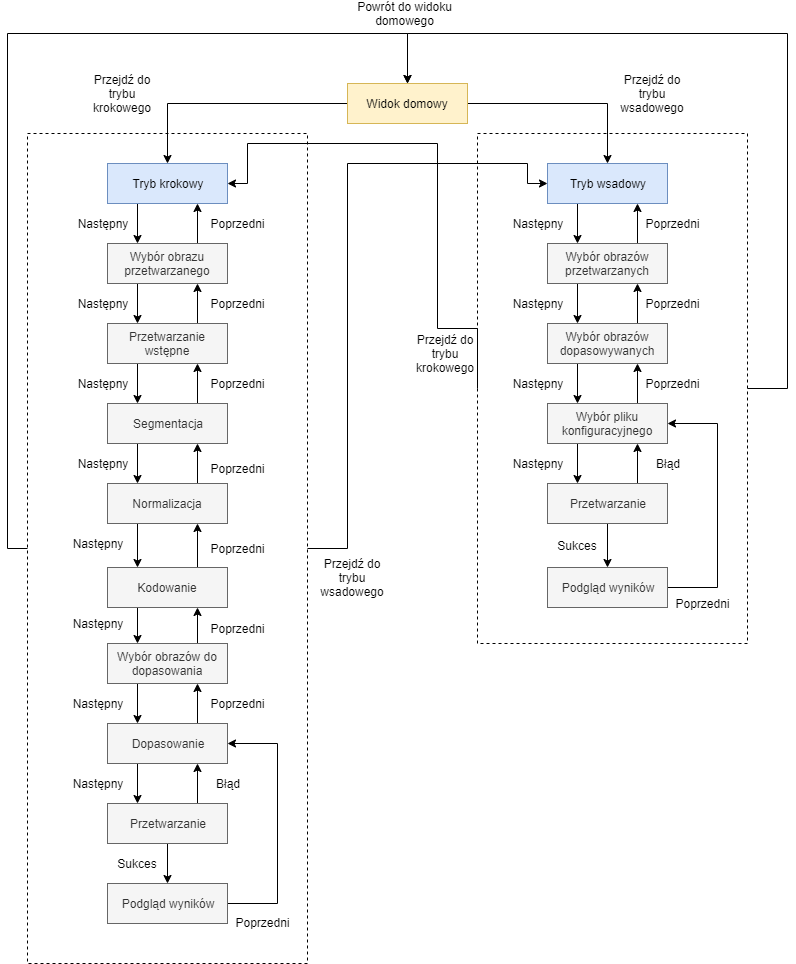
\includegraphics[width=\textwidth,height=\textheight, keepaspectratio]{images/widokiMgr.png}
    \caption{Diagram widoków i przejś\'c aplikacji.}
\end{figure}
